%\documentclass[openany]{book}
\documentclass[12pt]{article}
\usepackage[utf8]{inputenc}
\usepackage{amssymb} %for fancy L
\usepackage{calrsfs} %for fancy L
\usepackage{cancel}
\usepackage{tabularx}
\usepackage[hyphens]{url}
\usepackage{booktabs}
\usepackage{graphicx}
\usepackage[titletoc,title]{appendix}
\usepackage{subfig}
\DeclareMathAlphabet{\pazocal}{OMS}{zplm}{m}{n} %for fancy L
\usepackage{epsfig, float,array,tabu,longtable,}
\usepackage{hyperref,wrapfig}
\usepackage{enumerate}
\usepackage{graphicx,psfrag}
\usepackage{cite}
\usepackage{sectsty}
\usepackage{epstopdf}
\usepackage{amsmath,esint, setspace, fancyhdr, amsfonts, bookmark, blindtext}
\usepackage[normalem]{ulem}
\usepackage{tikz}
\usepackage{rotating}
\usepackage[americanvoltages,fulldiodes,siunitx]{circuitikz}
\usepackage{stackengine}
\usetikzlibrary{matrix}
\usepackage{multirow}
\usepackage{multicol}
\usetikzlibrary{shapes,backgrounds,patterns}
\usetikzlibrary{mindmap,trees,decorations.markings}
\usetikzlibrary{quotes,angles}
\usepackage{verbatim}
\renewcommand{\baselinestretch}{1}
\setlength{\textheight}{8in}
\setlength{\textwidth}{6.5in}
\setlength{\headheight}{0in}
\setlength{\headsep}{0.25in}
\usepackage{graphicx}
\setlength{\topmargin}{0in}
\setlength{\oddsidemargin}{0in}
\setlength{\evensidemargin}{0in}
\setlength{\parindent}{.3in}
\usepackage{listings}
\usepackage{color} %red, green, blue, yellow, cyan, magenta, black, white
\definecolor{mygreen}{RGB}{28,172,0} % color values Red, Green, Blue
\definecolor{mylilas}{RGB}{170,55,241}
\doublespacing
\begin{document}


\begin{titlepage}

\newcommand{\HRule}{\rule{\linewidth}{0.5mm}} % Defines a new command for the horizontal lines, change thickness here

\center % Center everything on the page
 
%---------------------------------------------------------
%	HEADING SECTIONS
%---------------------------------------------------------

\textsc{\LARGE Colorado School of Mines}\\[1.5cm] % Name of your university/college
\textsc{\Large CSCI 444}\\[0.5cm] % Major heading such as course name
\textsc{\large Advanced Computer Graphics}\\[0.5cm] % Minor heading such as course title

%---------------------------------------------------------
%	TITLE SECTION
%---------------------------------------------------------

\HRule \\[0.6cm]
{ \huge \bfseries 2D Procedural Heightmap Generation with Randomized Biomes}\\[0.4cm] % Title of your document
\HRule \\[1.0cm]
 
%---------------------------------------------------------
%	AUTHOR SECTION
%---------------------------------------------------------

\begin{minipage}{0.4\textwidth}
    \begin{flushleft}
        \emph{Author:}  
        \medskip
        {\textsc{\textbf{Robinson Merillat }}}   % Your name, bold and small caps    
    \end{flushleft}
\end{minipage}
\begin{minipage}{0.45\textwidth}
    \begin{flushright} \large
        \emph{Supervisor:}
        {\textsc{\textbf{Dr. Jeffery Paone }}} % Supervisor's Name
    \end{flushright}
\end{minipage}\\[1cm]

%---------------------------------------------------------
%	DATE SECTION
%---------------------------------------------------------
\begin{center}
{\large \today}
\end{center}
 % Date, change the \today to a set date if you want to be precise

%---------------------------------------------------------
%	LOGO SECTION
%---------------------------------------------------------
%\vfill
\newcommand*{\plogo}{
\includegraphics[width=0.25\textwidth]{../project_proposal/imgs/mines.png}}

\plogo\\[1cm] % Include a department/university logo - this will require the graphicx package
 
%---------------------------------------------------------

\vfill % Fill the rest of the page with whitespace
\end{titlepage}

\newpage

\section{abstract}
    The purpose of this project is to explore procedural terrain generation, creating a realistic and believable terrain 
    while attempting to conserve system memory and process time to prevent visible frame drop. I used a two pass technique
    storing computing a 2D noise texture in the first pass and using it in displacement mapping in the vertex shader of the
    second pass (heightmapping). Using several noise algorithms in continuum, I was able to reduce the number of octaves
    needed and still create a believable and interesting environment. A lot could be done to improve this project however,
    I am very happy with how it turned out and what I leaned about noise algorithms in the process.

\newpage

\tableofcontents

\section{Introduction}
    \subsection{background}
        Procedural Generation: "A method of creating data algorithmically as opposed to manually". [wikipedia]

        Procedural generation has been around almost as long as computing has. It has been used to generate sample data, 
        create music, and in computer graphics is often used to generate textures and object meshes. Modern video games 
        often take advantage of this method to create randomized environments and events in order to maintain player interest.
        This method has several advantages over stored data including smaller file sizes, a greater amount of content, 
        and a less predictable system.

        Procedural Terrain Generation is a subsection of procedural generation that focuses on manipulating
        a mesh to create terrain that simulates a real or fantasy like world. It involves most visual aspects a biome 
        including flora, and fauna.

        Procedural generation works extremely well for terrain because, as we have found out, nature itself follows 
        mathematical equations and isn't truly completely random. Trees bunch together and grow where water flows,
        erosion is a function of time. Plants grow in fractal like patterns. Each of these examples can are mathematical 
        equations that can be manipulated to create a repeatable pattern.

    \subsection{Intro}

        Procedural Terrain Generation (PTG) is the culmination of everything that fascinates me; the way that Biology and 
        Physics work together and using algorithms to study the relationships between them. Not only is this subject a 
        personal interest of mine, but it is also heavily used in many industries, most heavily of which is the gaming 
        industry. Many games with repetitive gameplay require procedural terrain to keep things interesting for the player. 
        Each time you load into a map on Diablo you aren't quite sure where that one cave is going to be, or if it'll 
        even show up at all. This kind of unknown exploration is what keeps players playing.  Aside from games; PTG is 
        also used in space programs to model the surface of nearby celestial bodies, allowing for simulations to be run 
        for new technologies.

        The difficulty of PTG comes in two forms. The first of which is integrating several algorithms together to where 
        the output of one becomes the input to another and so on for as many algorithms as you'd like to use. Secondarily 
        is determining just how the data should be manipulated to generate a realistic, desirable, result.  Just how much 
        should ridges be sharpened and peaks be weathered? What weight should each of the algorithms have? And in which 
        order should they be used to get a result that looks and feels right?

        The primary goal that I had for this project is to begin to understand how the various algorithms manipulated 
        the terrain and how I can efficiently utilize them to create terrains that I would want to explore as a 
        player within a game.

\section{Previous Works}
    As previously mentioned, PTG is not a new techniques, not is it one that has been entirely flushed out. Below are several 
    works that have inspired and instructed me on my path of discovering PTG.

    \subsection{Designer Worlds: Procedural Generation of Infinite Terrain from Real-World Elevation Data}

        This research paper delves into sending real world geographical elevation data into a variation of the perlin 
        noise algorithm called value noise. The geographical data used is from the United States Geological Survey of Utah.
        The value noise algorithm differs from the noise algorithm in that it chooses a randow height to interpolate between 
        as opposed to the gradients. Additionally value noise isn't contrained to be zero at grid points. It has a small speedup 
        over perlin noise, however this is only visible at higher dimensions. [Parberry]

    \subsection{Realtime Procedural Terrain Generation}

        This paper provides an overview of erosion techniques used in games for terrain synthesis. It also goes into 
        detail on how basic perlin noise is inferrior to voronoi diragrams. The 2D texture is then perturbed. Afterwards, 
        seperate erosion techniques can be used such as thermal erosion, Hydraulic erosion, or an algorithm that the writers 
        propose that combines the advantages of the two previously mentioned algorithms. [Olsen]

    \subsection{GDC talk on Building worlds with Noise Gerneration in No Man's Sky}

        This video clip from the Game Developer's Conference in March of 2017 discusses the techniques used by the 
        developers of No Man's Sky to procedurally generate an entire univers in no more than 300MB of code, and 200GB of 
        pre-developed assets. They create their own generation technique using a new noise method dubbed Uber Noise by 
        the speaker Sean Murray. It combines several noise methods including Analytical derivative and domain warping. [Murray]

\section{Problem Statement}

    Many of the traditional programs and methods of terrain generation take into account large amounts of system Memory
    as most dedicated graphics cards (GPU) have their own memory. However, for an Integrated GPU, like that on a Macintosh laptop,
    the onboard GPU steals from the computers' RAM rather than its own. This oftentimes prevents running heavy graphical 
    software such as high performance games on these laptops. The purpose of this project is to explore procedural terrain
    generation, creating a realistic and believable terrain while attempting to conserve system memory and process time
    to prevent visible frame drop.

    \subsection{Project Scope}
        Throughout the development of this program, it was quickly obvious that many of the stretch goals that I would 
        have liked to add were not within the scope of this project due to the various time constraints. Many of the goals
        and stretch goals of this project involved understanding the algorithms that can create believable biomes. 
        Each of which is on its' own a Master's thesis worth of understanding. As such I decided to forego some of these
        investigations until I had more time to sit down and understand the material.

\section{Problem Solution}
    The solution that I came up with require a lot of trial and error testing, along with hours of searching for better,
    more efficient noise algorithms. Using openGL 3.3+ in c++ I created a two pass method that generated the noise
    texture on the first pass through the rendering pipeline, and then generated the terrain on the second pass. I used 
    a Frame Buffer Object (FBO) to store the results of the first pass' fragment shader to a 2D texture. This texture was 
    then used in the vertex shader of the second pass to perform displacement mapping. This technique uses the RGB values 
    of the texture to distort a mesh. In this case, I was using a form of displacement mapping called Hightmapping. This 
    technique sets the y(vertical) value of each vertex equal to a scalar * the color at that vertex on the noise texture.
    As the texture is black and white, a range of heights can be computed, 0 being pure black and 1 being pure white. The 
    scalar value then perturbs the height to accentuate or diminish the features. 

    Several noise algorithms are defined in the fragment shader of the first pass such as: Classic Perlin Noise, 
    Voronoi (Cell) Noise, Fractal Brownian Motion, Ridged Noise, Billowed Noise, and Erosion Noise. Using these algorithms,
    I constructed several "biome" functions that utilized a different combinateion for these algorithms in order to simulate 
    the related biome. I implimented an Island, Mountain, Canyon/Desert, and Rugged terrain function. A randomized value
    seeded on the current system clock is sent into the shader as a uniform and that determines which biome is generated.
    Additionally, a few other pre-computed random values are sent in as scalars to the various noise algorithms. This gives
    a small amount of randomization, however, it is often times not a very visible differnece from one generation to another.

\section{Results}
    Testing for this project was performed on an Apple Macbook Pro(Retina, 13-inch, Late 2012). It has a 2.5GHz Intel Core i5
    processor, 8Gb of 1600MHz DDR3 RAM, and an Intel HD Graphics 4000 1536Mb onboard GPU. Using this device let me test on a 
    system that a typical user may use, at least as far as the processor and GPU. This means that if the program runs well
    on this device, chances are it'll run great on a newer or better spec'd device. 

    I had to run several iterations and tests of simply modifying scalars and changing the order of different noise algorithms
    get desired effects for each biome, however, in the end, I believe that I have created some relatively believable 
    terrains that run smoothly on the tested computer.

    \vspace{1cm}
    \begin{center}
        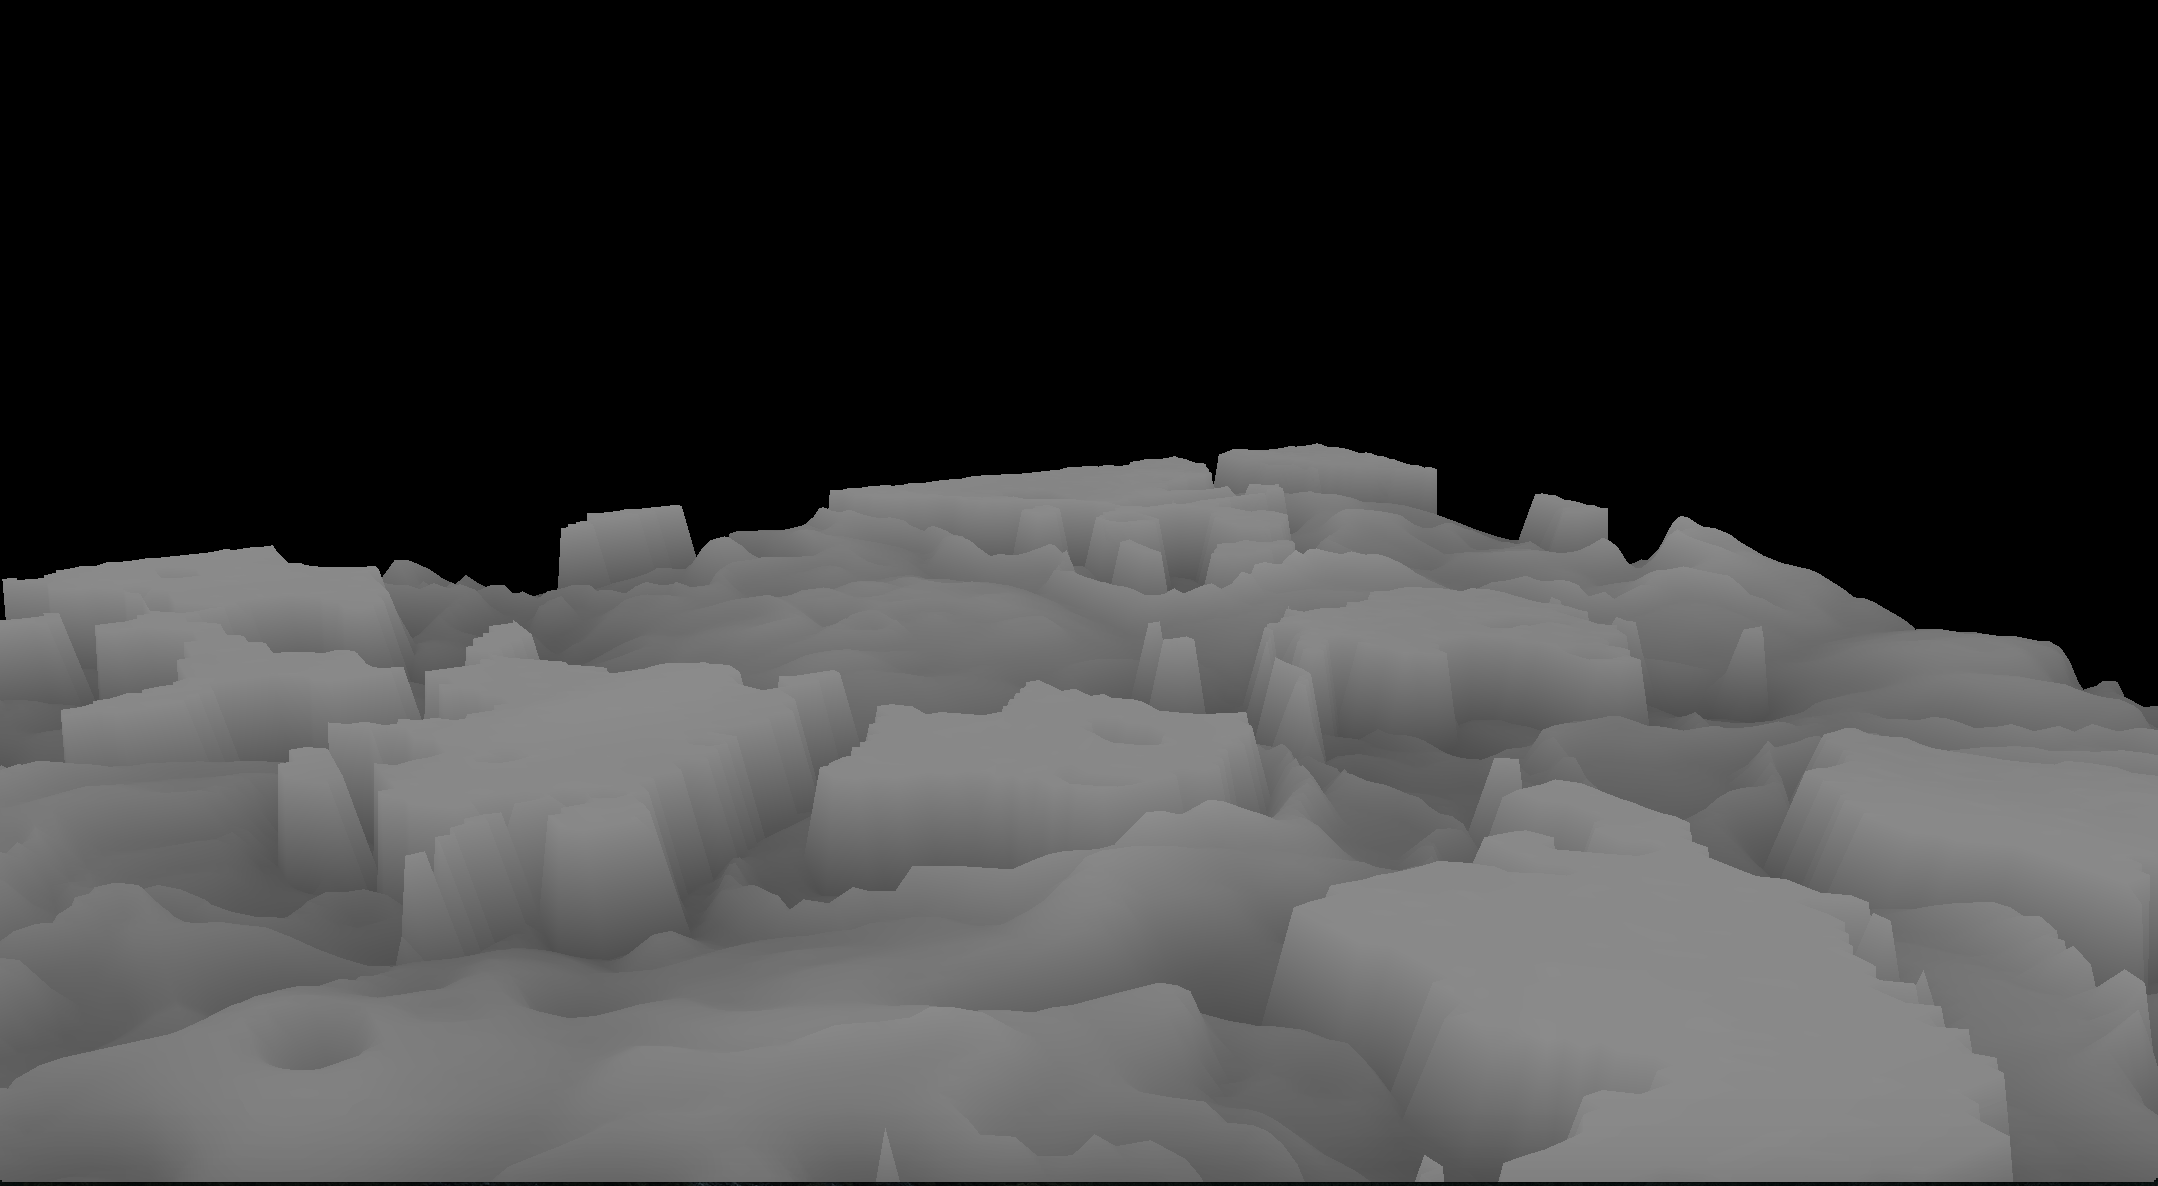
\includegraphics[width=0.75\textwidth]{images/1.png} 
    \end{center}
    
    Using a combination of several algorithms allowed me to keep the number of octaves used in the noise algorithms low. This 
    is helped by the scale and perspective of the view. If I were on the surface of the terrain, I may want the octaves to
    be higher to generate more close up detail, however, from far away, fewer octaves are necessary, especially if you added
    surface normals and decent lighting. 

\section{Conclusion}

    This project was a lot of fun, but very complex for me. Although I love them, I have trouble understanding algorithms and
    how they can be manipulated. As such I likely spent more time than was necessary of fiddling with the various algorithms
    and trying to get them to work.

    If I were to do this project again, I would most certainly start by loading in a low poly model and trying to get a
    Tessellation shader working to create a level of detail as this can save a lot of processing power. I would have also implimented 
    better lighting and textures to make the terrain look more appealing than a bunch of black and white textures.

    \section{Future Work}
        I plan to continue with this project in an attempt of increasing both the complexity and the performance.
        Some of the methods in which I may increase the performance may be to convert the mesh to be drawn as a Triangle Strip,
        conserving valuable vertices. Pre-determining which fragments will be in view and discarding them, and using Tessellation 
        Shaders to implement a Level of Detail hierarchy to render low poly far away and high poly close up to the camera.
        Complexity wise, I would like to get more randomized and versatile noise algorithms. I would also like to use more accurate 
        erosion algorithms and investigate procedurally populating each terrain with low poly flora and fauna.
        Lastly, I would like to implement using 3D noise with voxels to create more randomizes and interesting terrain.

        I would like to turn this from just a 2D terrain generation simulation in 3D into a 3D ecosystem simulation in 4D (time).

\section{Sources} 
    \begin{enumerate}
        \item Procedural Generation, Wikipedia, \href{https://en.wikipedia.org/wiki/Procedural_generation}[Link].
        \item Ian Parberry, Designer Worlds: Procedural Generation of Infinite Terrain from Real-World Elevation Data, Journal of Computer Graphics Techniques (JCGT), vol. 3, no. 1, 74-85, 2014
        \item Olsen, J. (2018). Realtime Synthesis of Eroded Fractal Terrain for Use in Computer Games. [ebook] Available at: https://pdfs.semanticscholar.org/5961/c577478f21707dad53905362e0ec4e6ec644.pdf [Accessed 23 Mar. 2018]. 
        \item Smelik, R., Tutenel, T., Bidarra, R. and Benes, B. (2014). A Survey on Procedural Modelling for Virtual Worlds. Computer Graphics Forum, 33(6), pp.31-50.
        \item Sean Murray GDC-Talk (2017) | Building Worlds with Noise Generation | No Man's Sky. (2017). [video] Game Developer's Conference \href{https://www.youtube.com/watch?v=SePDzis8HqY}{Link}
        \item Vivo, Patricio Gonzolez, The Book of Shaders, GLSL-noise Implimentations \href{https://gist.github.com/patriciogonzalezvivo/670c22f3966e662d2f83}[Github]
    \end{enumerate}  

\end{document}